\documentclass[12pt, a4paper, oneside]{article} % Paper size, default font size and one-sided paper
%\graphicspath{{./Figures/}} % Specifies the directory where pictures are stored
%\usepackage[dcucite]{harvard}
\usepackage{amsmath}
\usepackage{setspace}
\usepackage{pdflscape}
\usepackage{rotating}
\usepackage[flushleft]{threeparttable}
\usepackage{multirow}
\usepackage[comma, sort&compress]{natbib}% Use the natbib reference package - read up on this to edit the reference style; if you want text (e.g. Smith et al., 2012) for the in-text references (instead of numbers), remove 'numbers' 
\usepackage{graphicx}
%\bibliographystyle{plainnat}
\bibliographystyle{agsm}
\usepackage[colorlinks = true, citecolor = blue, linkcolor = blue]{hyperref}
%\hypersetup{urlcolor=blue, colorlinks=true} % Colors hyperlinks in blue - change to black if annoying
%\renewcommand[\harvardurl]{URL: \url}
\begin{document}
\title{Stats and Probability Information}
\author{Rob Hayward}
\date{\today}
\maketitle
\subsection*{Continuous and marginal distributions}

The marginal distribution of $x$ in a two-variable distribution is equal to the sum of the joint distribution over $y$. 
\begin{equation}
Pr(X = x) = \sum_y Pr(X = x, Y = y) = \sum_y Pr(X = x|Y = y)Pr(Y = y)
\end{equation}

From \href{http://en.wikipedia.org/wiki/Marginal_distribution}{Wikipedia}

For the continuous case
\begin{equation}
p_X(x) = \int_y p_{X,Y}(x,y)dy = \int_y p_{X|Y}(x|y)p_Y(y)dy
\end{equation}

There are three related distributions:  the marginal, the joint and the conditional. 

\subsection{Markov Chain Monte Carlo Methods}
This comes from Dave Miles.  There are four sections. 
\begin{itemize}
\item \href{http://davegiles.blogspot.ca/2014/03/mcmc-for-econometrics-students-i.html}{Introduction}
\item \href{http://davegiles.blogspot.ca/2014/03/mcmc-for-econometrics-students-ii_18.html}{Showing the MCMC works}
\item \href{http://davegiles.blogspot.ca/2014/03/mcmc-for-econometrics-students-iii.html}{Example to extract the marginal posterior distribution}
\item \href{http://davegiles.blogspot.com/2014/03/mcmc-for-econometrics-students-part-iv.html#more}{Use R to implement MCMC}
\end{itemize}

This is an update of the code by \href{http://www.econometricsbysimulation.com/2014/04/dave-giles-on-mcmc-for-econometrics.html}{Economics by Simulation}

The Gibbs sampler exploits the characteristics of the Markov chain.  With two parameters $\theta_1$ and $\theta_2$, $p(\theta_1, \theta_2)$ is the prior pdf and $L(\theta_1, \theta_2 | y) = p(y | \theta_1, \theta_2$ is the likelihood function.  Using Bayes theory, the posterior pdf for the parameters is 
\begin{equation}
p(\theta_1, \theta_2| y) \propto p(\theta_1, \theta_2)L(\theta_1, \theta_2| y)
\end{equation}

There are a numbrer of steps. 
\begin{enumerate}
\item Assign initial values to $\theta_1^{(0)}$ and $\theta_2^{(0)}$
\item Draw a random value $\theta_1^{(1)}$ from $p(\theta_1|\theta_2^{(0)}, y)$
\item The draw a random value $\theta_2^{(1)}$ from $p(\theta_2|\theta_1^{(1)}, y)$
\item Draw a random value $\theta_1^{(2)}$ from $p(\theta_1|\theta_2^{(1)}, y)$
\item Repeat items 3 and 4
\end{enumerate}

We end up a with two series that are Markov chains so the initial values do not matter and after many replications the chains start to behave as if they were random draws from the \emph{marginal} posterior distibution $p(\theta_1 |y)$ and $p(\theta_2|y)$ rather than the \emph{conditional} posterior distribution $p(\theta_1| \theta_2, y)$ $p(\theta_1|\theta_2, y)$.  The early values are part of the \emph{burn in} period and should be discarded.   

Here is a very simple version of the sampler applied to linear regression.  A draw for the slope coefficient is made conditional upon the given intercept and then a new intercept is drawn conditional on the slope.  This is repeated.  I think that they should be random draws from the data.  

\begin{knitrout}
\definecolor{shadecolor}{rgb}{0.969, 0.969, 0.969}\color{fgcolor}\begin{kframe}
\begin{alltt}
\hlcom{# Create a simple MCMC sampler}

\hlstd{x} \hlkwb{<-} \hlkwd{seq}\hlstd{(}\hlnum{1}\hlstd{,} \hlnum{100}\hlstd{,} \hlkwc{by} \hlstd{=} \hlnum{1}\hlstd{)}
\hlstd{e} \hlkwb{<-} \hlkwd{rnorm}\hlstd{(}\hlkwd{length}\hlstd{(x))}
\hlstd{y} \hlkwb{<-} \hlnum{0.5} \hlopt{+} \hlnum{5} \hlopt{*} \hlstd{x} \hlopt{+} \hlstd{e}
\hlcom{# prior }
\hlstd{a} \hlkwb{<-} \hlkwd{rep}\hlstd{(}\hlnum{NA}\hlstd{,} \hlkwc{times} \hlstd{=} \hlkwd{length}\hlstd{(x))}
\hlstd{b} \hlkwb{<-} \hlkwd{rep}\hlstd{(}\hlnum{NA}\hlstd{,} \hlkwc{times} \hlstd{=} \hlkwd{length}\hlstd{(x))}
\hlstd{a[}\hlnum{1}\hlstd{]} \hlkwb{=} \hlnum{1}
\hlstd{b[}\hlnum{1}\hlstd{]} \hlkwb{=} \hlnum{1}
\hlkwa{for}\hlstd{(i} \hlkwa{in} \hlnum{2}\hlopt{:}\hlnum{100}\hlstd{)\{}
\hlstd{b[i]} \hlkwb{<-} \hlstd{(y[i]} \hlopt{-} \hlstd{a[i}\hlopt{-}\hlnum{1}\hlstd{]} \hlopt{-} \hlkwd{rnorm}\hlstd{(}\hlnum{1}\hlstd{))}\hlopt{/}\hlstd{x[i]}
\hlstd{a[i]} \hlkwb{<-}  \hlstd{y[i]} \hlopt{-} \hlstd{b[i]}\hlopt{*}\hlstd{x[i]} \hlopt{-} \hlkwd{rnorm}\hlstd{(}\hlnum{1}\hlstd{)}
\hlstd{\}}
\hlkwd{plot}\hlstd{(y} \hlopt{~} \hlstd{x,} \hlkwc{type} \hlstd{=} \hlstr{'p'}\hlstd{,} \hlkwc{main} \hlstd{=} \hlstr{"Regression with OLS (red) and MCMC (blue)"}\hlstd{)}
\hlkwd{abline}\hlstd{(}\hlkwc{a} \hlstd{=} \hlkwd{mean}\hlstd{(a),} \hlkwc{b} \hlstd{=} \hlkwd{mean}\hlstd{(b),} \hlkwc{col} \hlstd{=} \hlstr{'blue'}\hlstd{)}
\hlkwd{lines}\hlstd{(}\hlkwd{fitted}\hlstd{(}\hlkwd{lm}\hlstd{(y} \hlopt{~}\hlstd{x)),} \hlkwc{col} \hlstd{=} \hlstr{'red'}\hlstd{)}
\end{alltt}
\end{kframe}
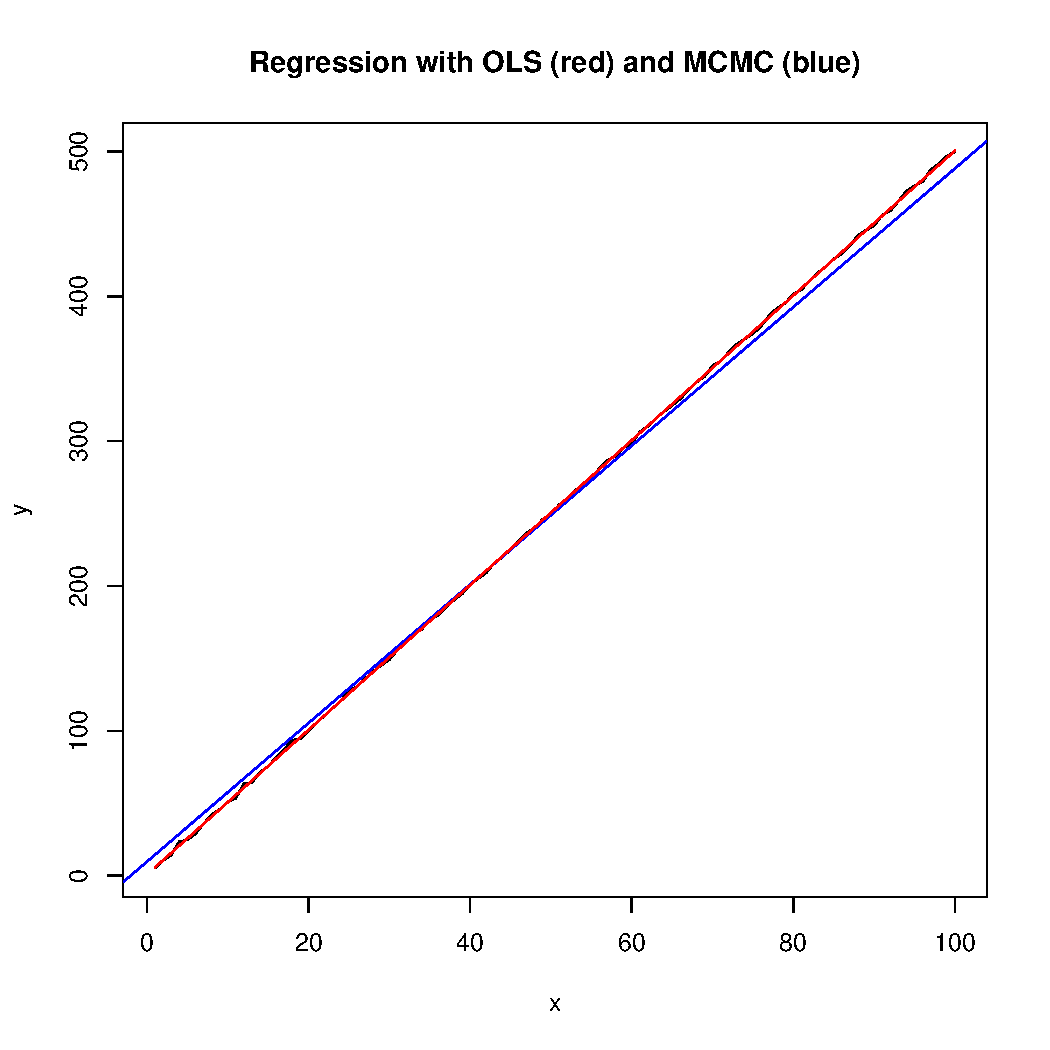
\includegraphics[width=\maxwidth]{figure/MCMC} 

\end{knitrout}

Once there is a large sample of $p(\theta_1|y)$ and the burn-in have been discarded, the mean, variance, median or mode of the marginal posterior can be calculated.  The process can be expanded to more parameters. 

\subsubsection{Gibbs Sampler}
The Gibbs sampler is a special case of the Metropolis-Hasting algorithm. 
The R code from Dave Giles in the file DaveGilesMCMCcoes.R has better version than this. I am not sure how we got from $\rho = 0.5$ to $sd = 1-\rho^2$. 

This example is based on two random variables $Y_1$ and $Y_2$, with a mean vector of $(\mu_1, \mu_2)$ a correlation of $\rho$, the variances of $Y_1$ and $Y_2$ are $\sigma_1^2$ and $\sigma_2^2$ respectively and the covariance between $Y_1$ and $Y_2$ is $\rho \sigma_1 \sigma_2$. \footnote{As $\rho = \frac{\sigma_{Y_1, Y_2}}{\sigma_1 \sigma_2}$.  Some additional reading on covariance \href{http://www.cogsci.ucsd.edu/~desa/109/trieschmarksslides.pdf}{http://www.cogsci.ucsd.edu/~desa/109/trieschmarksslides.pdf}}



The conditional distribution of $Y_1$ given $Y_2$ is 

\begin{equation}
p(Y_1| Y_2) \sim N \left(\mu_1 + \frac{\rho\sigma_1(Y_2 - \mu_2)}{\sigma_2}, \sigma_1^2(1 - \rho^2)\right)
\end{equation}

and the conditional distribution of $Y_2$ given $Y_1$ is

\begin{equation}
p(Y_2| Y_1) \sim N \left(\mu_2 + \frac{\rho\sigma_2(Y_1 - \mu_1)}{\sigma_2}, \sigma_1^2(1 - \rho^2) \right)
\end{equation}

This can be used to find the marginal distribution. It is known that the marginal distribution for $Y_1$ is
\begin{equation}
p(Y_1) \sim N(\mu_1, \sigma_1^2)
\end{equation}

and for $Y_2$ is 
\begin{equation}
p(Y_2) \sim N(\mu_2, \sigma_2^2)
\end{equation}

However, to test the MCMC draw from the conditional to find the marginal (that we already know).  

Set $\mu_1 = 0$ and $\mu_2 = 0$ and $\sigma_1 = 1$ and $\sigma_2 = 1$

The steps for the Gibbs sampler are 
\begin{enumerate}
\item Chose an initial value for $Y_1$ called $Y_1^{(0)}$
\item Next, generate a random $Y_2$ value ($Y_2^{(0)})$ from $p(Y_2| Y_1^{(0)})$
\item Then, generte a new random $Y_1$ value (say $Y_1^{(1)})$ from $p(Y_1| Y_2^{(0)})$
\item Repeat steps 2 and 3 many times saving the strings of $Y_1$ and $Y_2$ values.
\item Throw away the first thousand or so values as they are draws from the \emph{conditional distribution}
\item Now the values from the marginal distribution of interest
\end{enumerate}

\begin{knitrout}
\definecolor{shadecolor}{rgb}{0.969, 0.969, 0.969}\color{fgcolor}\begin{kframe}
\begin{alltt}
\hlkwd{set.seed}\hlstd{(}\hlnum{123}\hlstd{)}
\hlstd{nreps} \hlkwb{<-} \hlnum{105000}
\hlstd{nb} \hlkwb{<-} \hlnum{5000}
\hlstd{yy1} \hlkwb{<-} \hlkwd{array}\hlstd{(, nreps)}
\hlstd{yy2} \hlkwb{<-} \hlkwd{array}\hlstd{(, nreps)}
\hlstd{rho} \hlkwb{<-} \hlnum{0.5}
\hlstd{sd} \hlkwb{<-} \hlkwd{sqrt}\hlstd{(}\hlnum{1} \hlopt{-} \hlstd{rho}\hlopt{^}\hlnum{2}\hlstd{)}
\hlstd{y1} \hlkwb{<-} \hlkwd{rnorm}\hlstd{(}\hlnum{1}\hlstd{,} \hlnum{0}\hlstd{, sd)}
\hlkwa{for}\hlstd{(i} \hlkwa{in} \hlnum{1}\hlopt{:}\hlstd{nreps)\{}
  \hlstd{y2} \hlkwb{<-} \hlkwd{rnorm}\hlstd{(}\hlnum{1}\hlstd{,} \hlnum{0}\hlstd{, sd)} \hlopt{+} \hlstd{rho}\hlopt{*}\hlstd{y1}
  \hlstd{y1} \hlkwb{<-} \hlkwd{rnorm}\hlstd{(}\hlnum{1}\hlstd{,} \hlnum{0}\hlstd{, sd)} \hlopt{+} \hlstd{rho}\hlopt{*}\hlstd{y2}
  \hlstd{yy1[i]} \hlkwb{<-} \hlstd{y1}
  \hlstd{yy2[i]} \hlkwb{<-} \hlstd{y2}
\hlstd{\}}
\hlstd{nb1} \hlkwb{<-} \hlstd{nb} \hlopt{+} \hlnum{1}
\hlstd{yy1b} \hlkwb{<-} \hlstd{yy1[nb1}\hlopt{:}\hlstd{nreps]}
\hlstd{yy2b} \hlkwb{<-} \hlstd{yy2[nb1}\hlopt{:}\hlstd{nreps]}
\hlkwd{plot}\hlstd{(yy1b,} \hlkwc{col} \hlstd{=} \hlnum{2}\hlstd{,} \hlkwc{main} \hlstd{=} \hlstr{"MCMC for Bivarite Normal"}\hlstd{,} \hlkwc{xlab} \hlstd{=} \hlstr{"Repetitions"}\hlstd{,}
     \hlkwc{ylab} \hlstd{=} \hlstr{"Y1"}\hlstd{)}
\hlkwd{abline}\hlstd{(}\hlkwc{h} \hlstd{=} \hlnum{3}\hlstd{,} \hlkwc{lty} \hlstd{=} \hlnum{2}\hlstd{)}
\hlkwd{abline}\hlstd{(}\hlkwc{h} \hlstd{=} \hlopt{-}\hlnum{3}\hlstd{,} \hlkwc{lty} \hlstd{=} \hlnum{2}\hlstd{)}
\end{alltt}
\end{kframe}
\includegraphics[width=\maxwidth]{figure/MCM} 

\end{knitrout}
The values are centered around zero as they should be. 
\begin{knitrout}
\definecolor{shadecolor}{rgb}{0.969, 0.969, 0.969}\color{fgcolor}\begin{kframe}
\begin{alltt}
\hlkwd{plot}\hlstd{(yy2b,} \hlkwc{col} \hlstd{=} \hlnum{4}\hlstd{,} \hlkwc{main} \hlstd{=} \hlstr{"MCMC for Bivarite Normal"}\hlstd{,} \hlkwc{xlab} \hlstd{=} \hlstr{"Repetitions"}\hlstd{,}
     \hlkwc{ylab} \hlstd{=} \hlstr{"Y2"}\hlstd{)}
\hlkwd{abline}\hlstd{(}\hlkwc{h} \hlstd{=} \hlnum{3}\hlstd{,} \hlkwc{lty} \hlstd{=} \hlnum{2}\hlstd{)}
\hlkwd{abline}\hlstd{(}\hlkwc{h} \hlstd{=} \hlopt{-}\hlnum{3}\hlstd{,} \hlkwc{lty} \hlstd{=} \hlnum{2}\hlstd{)}
\end{alltt}
\end{kframe}
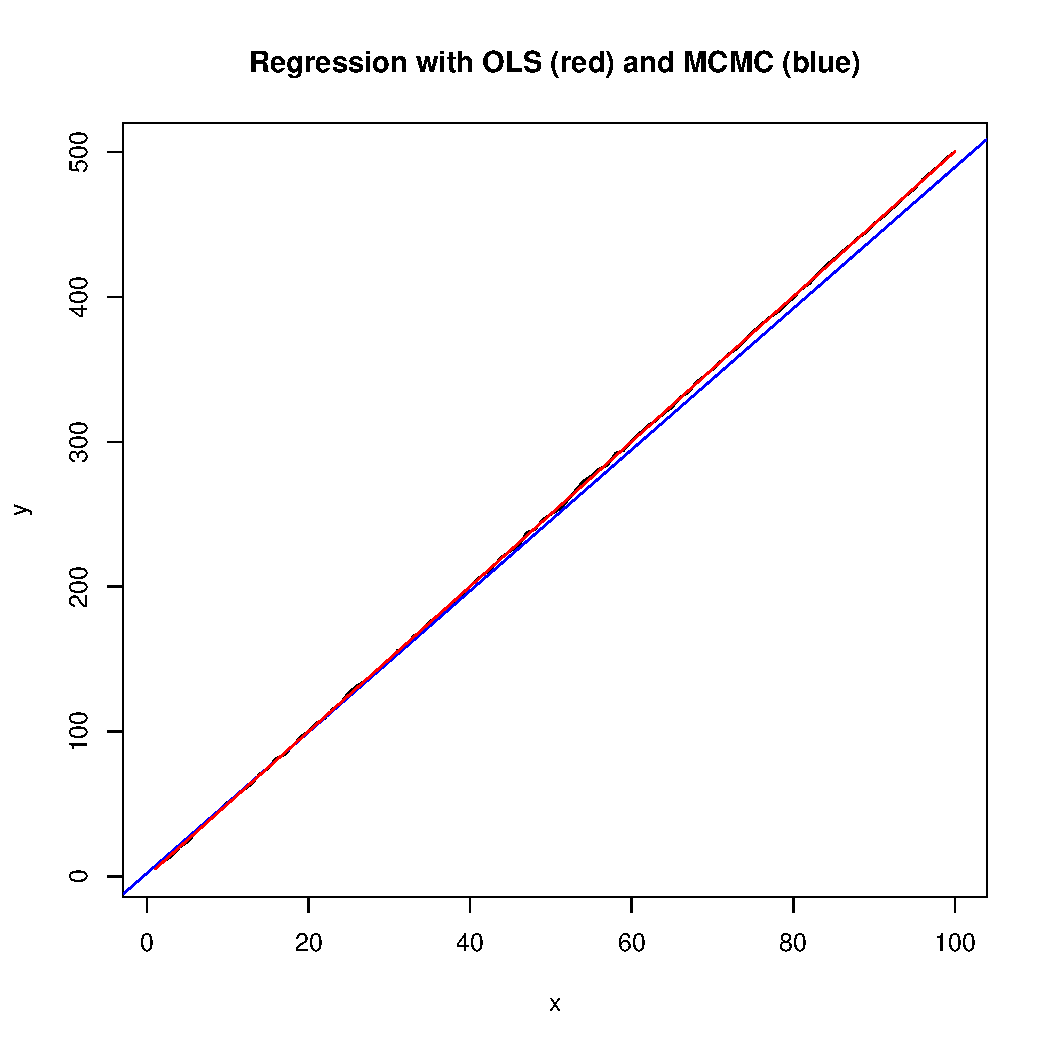
\includegraphics[width=\maxwidth]{figure/MCMC2} 

\end{knitrout}
The summary statistics are below. 
\begin{knitrout}
\definecolor{shadecolor}{rgb}{0.969, 0.969, 0.969}\color{fgcolor}\begin{kframe}
\begin{alltt}
\hlkwd{summary}\hlstd{(yy1b)}
\end{alltt}
\begin{verbatim}
##    Min. 1st Qu.  Median    Mean 3rd Qu.    Max. 
##  -4.400  -0.671   0.008   0.005   0.678   4.450
\end{verbatim}
\begin{alltt}
\hlkwd{var}\hlstd{(yy1b)}
\end{alltt}
\begin{verbatim}
## [1] 0.9954
\end{verbatim}
\begin{alltt}
\hlkwd{summary}\hlstd{(yy2b)}
\end{alltt}
\begin{verbatim}
##    Min. 1st Qu.  Median    Mean 3rd Qu.    Max. 
##  -4.280  -0.668   0.007   0.007   0.681   4.110
\end{verbatim}
\begin{alltt}
\hlkwd{var}\hlstd{(yy2b)}
\end{alltt}
\begin{verbatim}
## [1] 1.004
\end{verbatim}
\end{kframe}
\end{knitrout}
The means are zero and the variances are close  to unity. 

\begin{knitrout}
\definecolor{shadecolor}{rgb}{0.969, 0.969, 0.969}\color{fgcolor}\begin{kframe}
\begin{alltt}
\hlkwd{hist}\hlstd{(yy1b,} \hlkwc{prob} \hlstd{= T,} \hlkwc{col} \hlstd{=} \hlnum{2}\hlstd{,} \hlkwc{main} \hlstd{=} \hlstr{"MCMC for Bivariate Normal"}\hlstd{,} \hlkwc{xlab} \hlstd{=} \hlstr{"Y1"}\hlstd{,}
     \hlkwc{ylab} \hlstd{=} \hlstr{"Marginal PDF for Y1"}\hlstd{)}
\end{alltt}
\end{kframe}
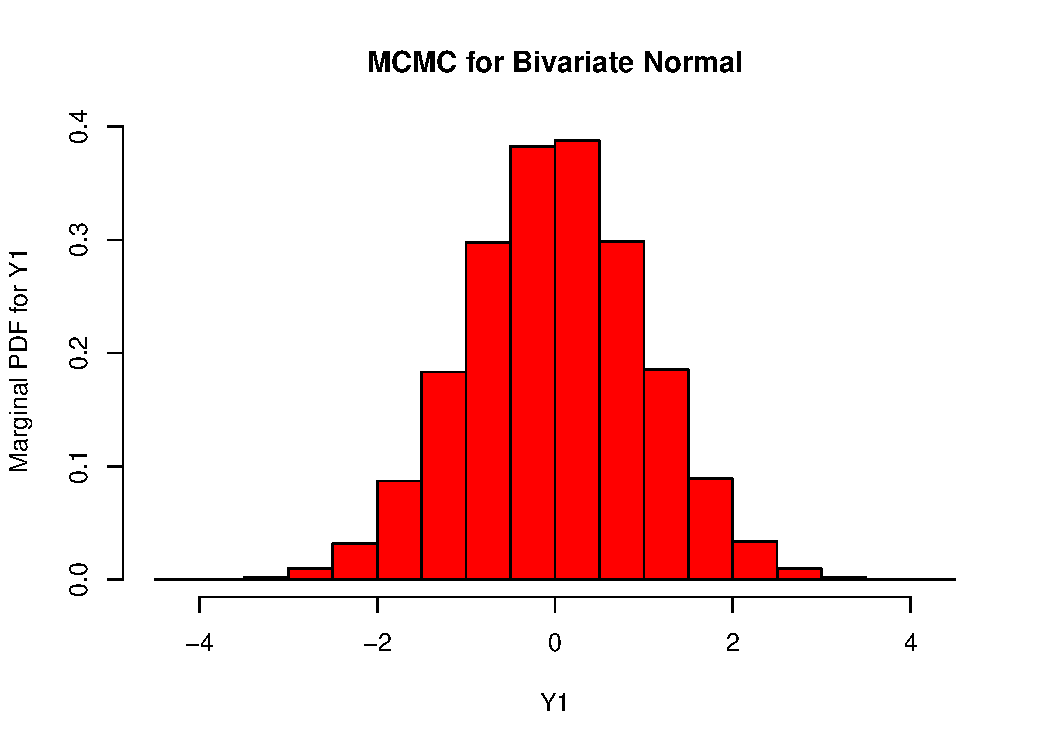
\includegraphics[width=\maxwidth]{figure/Hist1} 
\begin{kframe}\begin{alltt}
\hlkwd{hist}\hlstd{(yy2b,} \hlkwc{prob} \hlstd{= T,} \hlkwc{col} \hlstd{=} \hlnum{4}\hlstd{,} \hlkwc{main} \hlstd{=} \hlstr{"MCMC for Bivariate Normal"}\hlstd{,} \hlkwc{xlab} \hlstd{=} \hlstr{"Y2"}\hlstd{,}
     \hlkwc{ylab} \hlstd{=} \hlstr{"Marginal PDF for Y2"}\hlstd{)}
\end{alltt}
\end{kframe}
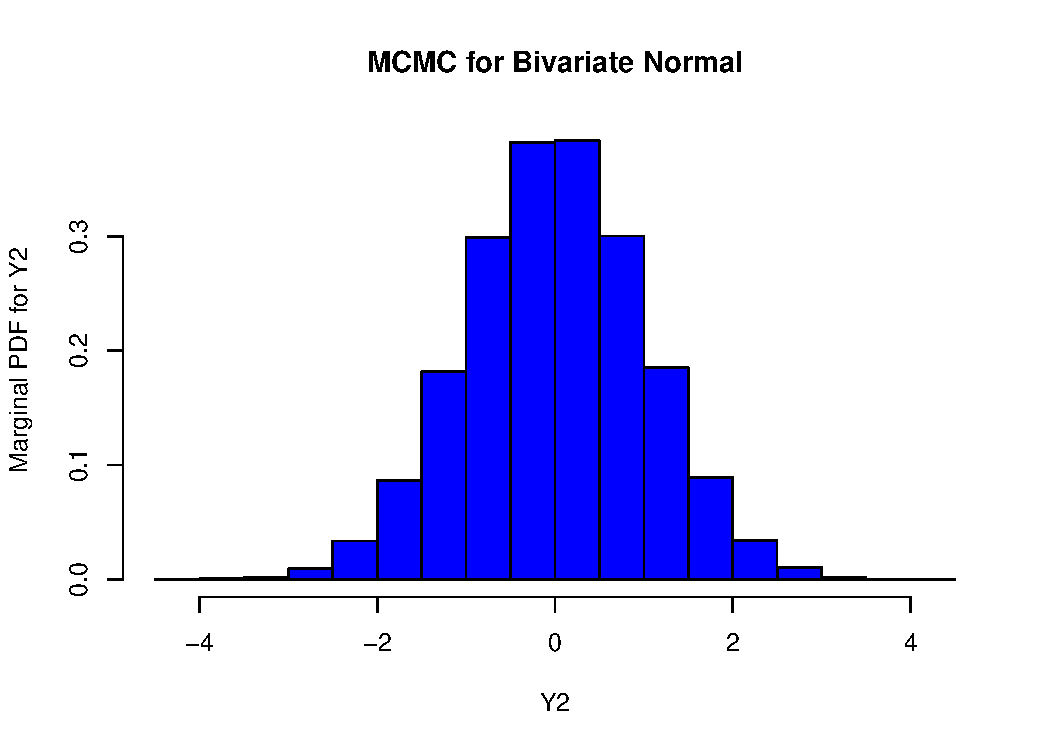
\includegraphics[width=\maxwidth]{figure/Hist2} 

\end{knitrout}

\begin{knitrout}
\definecolor{shadecolor}{rgb}{0.969, 0.969, 0.969}\color{fgcolor}\begin{kframe}
\begin{alltt}
\hlkwd{qqnorm}\hlstd{(yy1b)}
\end{alltt}
\end{kframe}
\includegraphics[width=\maxwidth]{figure/Tests1} 
\begin{kframe}\begin{alltt}
\hlkwd{qqnorm}\hlstd{(yy2b)}
\end{alltt}
\end{kframe}
\includegraphics[width=\maxwidth]{figure/Tests2} 
\begin{kframe}\begin{alltt}
\hlkwd{library}\hlstd{(tseries)}
\end{alltt}


{\ttfamily\noindent\bfseries\color{errorcolor}{\#\# Error: there is no package called 'tseries'}}\begin{alltt}
\hlkwd{jarque.bera.test}\hlstd{(yy1b)}
\end{alltt}


{\ttfamily\noindent\bfseries\color{errorcolor}{\#\# Error: could not find function "{}jarque.bera.test"{}}}\begin{alltt}
\hlkwd{jarque.bera.test}\hlstd{(yy1b)}
\end{alltt}


{\ttfamily\noindent\bfseries\color{errorcolor}{\#\# Error: could not find function "{}jarque.bera.test"{}}}\end{kframe}
\end{knitrout}

\subsubsection{Gibbs Sampler for Marginal Posterior}
Extract the \emph{marginal posterior distribution} from the \emph{joint posterior distribution}. Assume that there is a population with an unknown mean $\mu$ and an unknown precistion parameter $\tau$ where $\tau = 1/\sigma^2$. Before looking at the data we are \emph{a priori} ignorant about the possible values of the parameters, we assign the following joint pior density: 

\begin{equation}
p(\mu, \tau) = p(\mu) p(\tau) \propto 1/\tau ; \quad -\inf < \mu < \inf ; \quad 0 < \tau < \inf
\end{equation}

Now take a sample of n independent values from the population.  This will give a likelihood function of
\begin{equation}
L(\mu, \tau | y) = p(y | \mu, \tau) \propto \tau^{n/2} exp[-(\tau/2) \sum(y_i - \mu)^2]
\end{equation}

I do not understand the next step.  

Dave says that by Bayes law the \emph{joint} posterior density for the two parameters is
\begin{align}{\label{eqref:BL}}
p(\mu, \tau | y) &= [p(\mu, \tau)L(\mu, \tau | y)/ p(y)] \propto p(\mu, \tau)L(\mu, \tau |y)\\
                 &\propto \tau^{n/2 -1}exp[-(\tau/2)\sum(y_i - \mu)^2]
\end{align}

For the marginal densities it is necessary to input the conditional posterior densities into the Gibbs sampler.  
From Equation \ref{eqref:BL}, treat $\tau$ as a constant (so condition on $\tau$), 
\begin{align}
p(\mu | \tau, y) &\propto exp[-(\tau/2)\sum(y_i - \mu)^2]\\
&\propto exp[-(\tau/2) (vs^2 + \sum(\mu - y^*)^2)]\\
&\propto exp[-\tau/2)(\mu - y^*)^2]
\end{align}

where $y^*$ is the sample mean of $y$; $v = (n - 1)$; and $s^2$ is the sample variance. Therefore, the conditional posterior for $\mu$ is a normal distribution with a mean of $y^*$ and a variance of $(n\tau)^{-1}$.

Alternatively, if the conditioning is on $\mu$ 
\begin{equation}
p(\tau | \mu, y) \propto \tau^{n/2 -1}exp[-\tau(0.5\sum(y_i - \mu)^2)]
\end{equation}

So the conditional posterior for $\tau$ is a Gammer distribution with a shape parameter, $r = (n/2)$ and a scale parameter, $\lambda = [0.5\sum(y_i - \mu)^2]$. 

I do not understand the move to the conditional posterior and the distribution. 

Now implement the Gibbs Sampler
\begin{knitrout}
\definecolor{shadecolor}{rgb}{0.969, 0.969, 0.969}\color{fgcolor}\begin{kframe}
\begin{alltt}
\hlkwd{set.seed}\hlstd{(}\hlnum{123}\hlstd{)}
\hlcom{# MC replications}
\hlstd{nrep} \hlkwb{<-} \hlnum{105000}
\hlcom{# burn-in}
\hlstd{nb} \hlkwb{<-} \hlnum{5000}
\hlcom{# Sample size}
\hlstd{n} \hlkwb{<-} \hlnum{10}
\hlcom{# set up vectors}
\hlstd{tau} \hlkwb{<-} \hlkwd{array}\hlstd{(, nrep)}
\hlstd{mu} \hlkwb{<-} \hlkwd{array}\hlstd{(, nrep)}
\hlcom{# Create a sample of data.  true values are 1.}
\hlstd{y} \hlkwb{<-} \hlkwd{rnorm}\hlstd{(n,} \hlkwc{mean} \hlstd{=} \hlnum{1}\hlstd{,} \hlkwc{sd} \hlstd{=} \hlnum{1}\hlstd{)}
\hlstd{ybar} \hlkwb{<-} \hlkwd{mean}\hlstd{(y)}
\hlstd{yy} \hlkwb{<-} \hlkwd{sum}\hlstd{(y}\hlopt{^}\hlnum{2}\hlstd{)}
\hlstd{lambda} \hlkwb{<-} \hlnum{1}\hlopt{/}\hlstd{(}\hlnum{0.5} \hlopt{*} \hlstd{n} \hlopt{*} \hlkwd{var}\hlstd{(y))}
\end{alltt}
\end{kframe}
\end{knitrout}
Now create the loop for the Gibbs sampler
\begin{knitrout}
\definecolor{shadecolor}{rgb}{0.969, 0.969, 0.969}\color{fgcolor}\begin{kframe}
\begin{alltt}
\hlstd{ttau} \hlkwb{<-} \hlkwd{rgamma}\hlstd{(}\hlnum{1}\hlstd{,} \hlkwc{shape} \hlstd{= n}\hlopt{/}\hlnum{2}\hlstd{,} \hlkwc{rate} \hlstd{= lambda)}
\hlkwa{for}\hlstd{(i} \hlkwa{in} \hlnum{1}\hlopt{:}\hlstd{nrep)\{}
  \hlstd{mmu} \hlkwb{<-} \hlkwd{rnorm}\hlstd{(}\hlnum{1}\hlstd{,} \hlkwc{mean} \hlstd{= ybar,} \hlkwc{sd} \hlstd{=} \hlnum{1}\hlopt{/}\hlkwd{sqrt}\hlstd{(n}\hlopt{*}\hlstd{ttau))}
  \hlstd{scale} \hlkwb{<-} \hlstd{(}\hlnum{0.5} \hlopt{*} \hlstd{(yy} \hlopt{+} \hlstd{n} \hlopt{*} \hlstd{mmu}\hlopt{^}\hlnum{2} \hlopt{-} \hlnum{2} \hlopt{*} \hlstd{n} \hlopt{*} \hlstd{mmu} \hlopt{*} \hlstd{ybar))}
  \hlstd{ttau} \hlkwb{<-} \hlkwd{rgamma}\hlstd{(}\hlnum{1}\hlstd{,} \hlkwc{shape} \hlstd{= n}\hlopt{/}\hlnum{2}\hlstd{, scale)}
  \hlstd{tau[i]} \hlkwb{<-} \hlstd{ttau}
  \hlstd{mu[i]} \hlkwb{<-} \hlstd{mmu}
\hlstd{\}}
\end{alltt}
\end{kframe}
\end{knitrout}
Now drop the first 5000 values of $\mu$ and $\tau$ for the burn in. 
\begin{knitrout}
\definecolor{shadecolor}{rgb}{0.969, 0.969, 0.969}\color{fgcolor}\begin{kframe}
\begin{alltt}
\hlstd{nb1} \hlkwb{<-} \hlstd{nb} \hlopt{+}\hlnum{1}
\hlstd{taub} \hlkwb{<-} \hlstd{tau[nb1}\hlopt{:}\hlstd{nrep]}
\hlstd{mub} \hlkwb{<-} \hlstd{mu[nb1}\hlopt{:}\hlstd{nrep]}
\end{alltt}
\end{kframe}
\end{knitrout}
Take a look at the distributions for $\mu$ and $\tau$. They should be student-t (n-1) and Gamma respectively. 
\begin{knitrout}
\definecolor{shadecolor}{rgb}{0.969, 0.969, 0.969}\color{fgcolor}\begin{kframe}
\begin{alltt}
\hlkwd{require}\hlstd{(moments)}
\end{alltt}


{\ttfamily\noindent\itshape\color{messagecolor}{\#\# Loading required package: moments}}

{\ttfamily\noindent\color{warningcolor}{\#\# Warning: there is no package called 'moments'}}\begin{alltt}
\hlkwd{summary}\hlstd{(mub);} \hlkwd{var}\hlstd{(mub)}
\end{alltt}
\begin{verbatim}
##    Min. 1st Qu.  Median    Mean 3rd Qu.    Max. 
##  -2.760   0.863   1.080   1.070   1.290   3.960
## [1] 0.1161
\end{verbatim}
\begin{alltt}
\hlstd{ybar} \hlcom{# THe mean of the posterior for my should be ybar (1.0746)}
\end{alltt}
\begin{verbatim}
## [1] 1.075
\end{verbatim}
\begin{alltt}
\hlkwd{skewness}\hlstd{(mub)} \hlcom{# The skewness of student-t is zero}
\end{alltt}


{\ttfamily\noindent\bfseries\color{errorcolor}{\#\# Error: could not find function "{}skewness"{}}}\begin{alltt}
\hlkwd{kurtosis}\hlstd{(mub)} \hlcom{# THe excess kurtosis for student-t is 6/(n-5) = 1.2}
\end{alltt}


{\ttfamily\noindent\bfseries\color{errorcolor}{\#\# Error: could not find function "{}kurtosis"{}}}\begin{alltt}
\hlkwd{summary}\hlstd{(taub);} \hlkwd{var}\hlstd{(taub)}
\end{alltt}
\begin{verbatim}
##    Min. 1st Qu.  Median    Mean 3rd Qu.    Max. 
##   0.023   0.719   1.020   1.100   1.400   5.380
## [1] 0.2717
\end{verbatim}
\begin{alltt}
\hlkwd{skewness}\hlstd{(taub)} \hlcom{# the skewness of gamma is 2/sqrt(shape) = 0.8944}
\end{alltt}


{\ttfamily\noindent\bfseries\color{errorcolor}{\#\# Error: could not find function "{}skewness"{}}}\begin{alltt}
\hlkwd{kurtosis}\hlstd{(taub)} \hlcom{# excess kkurtosis of gamma is 6/(n/2) = 1.2}
\end{alltt}


{\ttfamily\noindent\bfseries\color{errorcolor}{\#\# Error: could not find function "{}kurtosis"{}}}\end{kframe}
\end{knitrout}

The last couple of comments from Dave are:
\begin{itemize}
\item The sample were drawn from a population with $\mu = \tau = 1$.  
\item With a quadratic loss function, the Bayes estimators of the parameters would be the marginal posterior means (see above). 
\item With an absolute error loss function, the Bayes estimators would be the marginal posterior medians. 
\end{itemize}
The marginal posterior densities. 

\begin{knitrout}
\definecolor{shadecolor}{rgb}{0.969, 0.969, 0.969}\color{fgcolor}\begin{kframe}
\begin{alltt}
\hlkwd{hist}\hlstd{(mub,} \hlkwc{main} \hlstd{=} \hlstr{"Marginal Posterior for mu:  Student-t"}\hlstd{,} \hlkwc{prob} \hlstd{=} \hlnum{TRUE}\hlstd{,} \hlkwc{col} \hlstd{=} \hlstr{"red"}\hlstd{)}
\end{alltt}
\end{kframe}
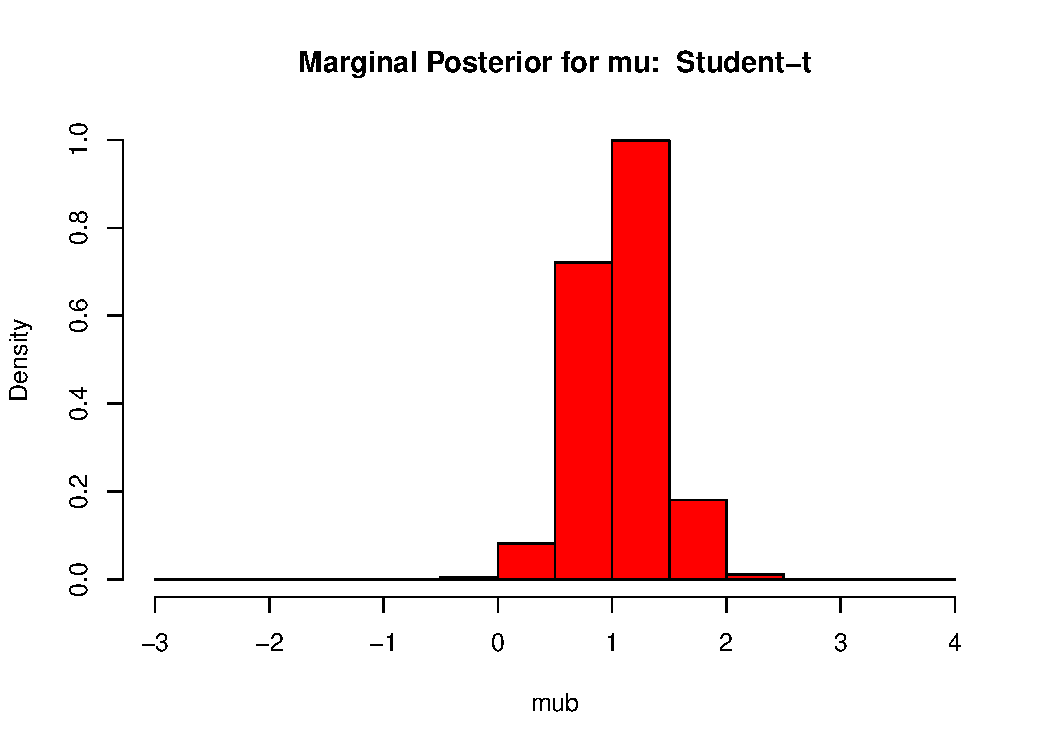
\includegraphics[width=\maxwidth]{figure/MCMCplot1} 
\begin{kframe}\begin{alltt}
\hlkwd{hist}\hlstd{(taub,} \hlkwc{main} \hlstd{=} \hlstr{"Marginal Posterior for tau: Gamma"}\hlstd{,} \hlkwc{prob} \hlstd{=} \hlnum{TRUE}\hlstd{,} \hlkwc{col} \hlstd{=} \hlstr{"blue"}\hlstd{)}
\end{alltt}
\end{kframe}
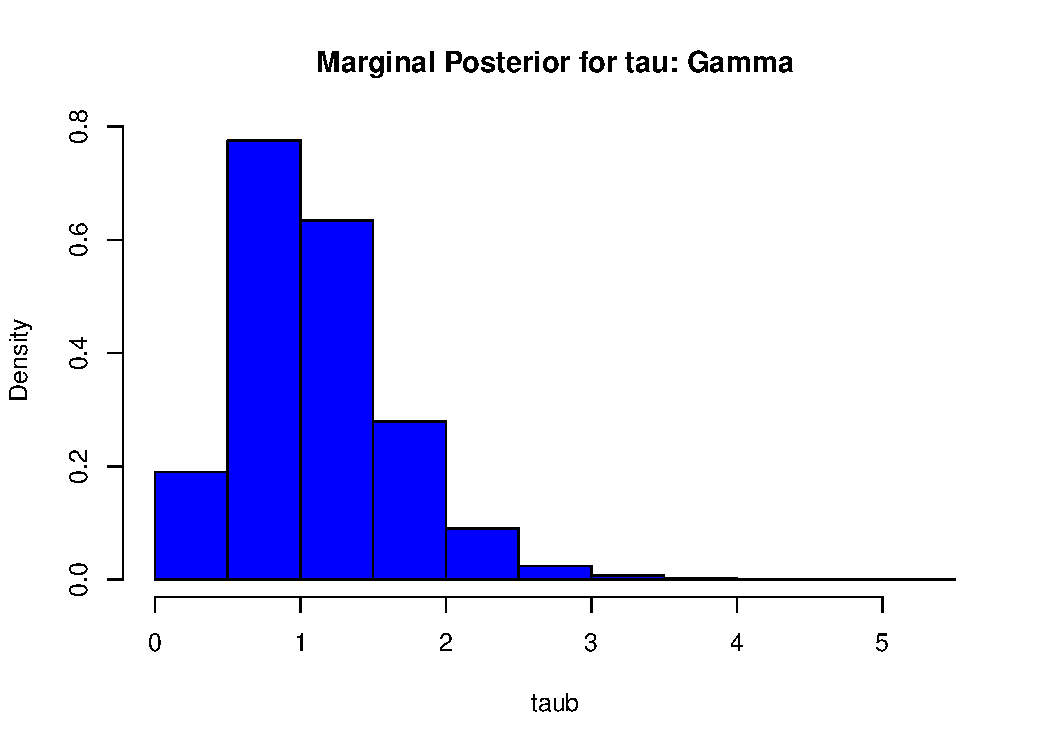
\includegraphics[width=\maxwidth]{figure/MCMCplot2} 

\end{knitrout}


\subsection{Mixture Model}
This is a probabilistic model that relates some random variables to some other variables.  The model has sub-populations. The properties of the sub-population are different from those of the parent. The sub-populations may not be observable.  For example, the distribution of returns may be different in different sub-population or regime. 

A \emph{mixture distribution} is the probability distribution of a random variable  whose values are derived from an underlying set of random variables. The \emph{mixture components} are individual distributions with \emph{mixture weights}.  Even in cases where the mixture comonents have a normal distribution, the mixture distribution is likely to be non-normal. Mixture models are used to understand the sub-population when there is only access to the information about the pooled population. 

The mixture model will be comprised of N random varibles distributed according to K components, with each component belonging to the same distribution. The k mixture weights sum to one. Each component will have parameters (mean and variance in the case of normal distribution).  

The method will try to estimate the all the parameters of the model from the data.  The underlying data is known $(x_i)$; the number of mixture components is set $(K)$; the parameters of the distribution of each mixture component $(\theta_{i=1\dots K})$; mixture weight $(\Phi_{i = 1\dots K})$; $\mathbf{\Phi}$ K-dimensional vector summing to 1; $F(x|\theta)$ probability distribution of observations parameterised on $\theta$; $\alpha$ shared hyperparameter for component weights; $\beta$ shared hyperparameter for mixture weights; $H(\theta|\alpha)$ prior probability distribution of component parameters; 


\subsection{Regression}
This is a series of sessions that introduce regression with R.  The first page is \href{http://pingax.com/2013/11/}{here}.  \href{http://pingax.com/linear-regression-with-r-step-by-step-implementation-part-1/}{Linear Regression: Step-by-step}. This is essentially a version of the Andrew Ng Machine Learning Course.  

If $Y$ is the dependent variable, $X_1, X_2, \dots X_n$ are the explanatory variables and $\Theta$ are unknown parameters, regression takes can be carried out in a number of ways. 

\subsubsection{OLS}
\begin{equation}
h_{\Theta}(x) = \Theta_0 + \Theta_1 x
\end{equation}

The aim is to find values of $\Theta$ so that the model will fit the data.  The \emph{cost function} will assess the difference between the predicted and the actual values. One version of the cost function is 
\begin{equation}
J(\Theta_0, \Theta_1) = \frac{1}{2m} \sum_{i=1}^m (h_{\Theta}(X^{(i)} - y^{(i)}))^2
\end{equation}
Change the values of $\Theta$ to minimise the cost. The method used is gradient decent. 

The partital derivative of the cost function with respect to the $\Theta$ are
\begin{subequations}
\begin{equation}
\Theta_0 = \Theta_0 - \alpha \frac{1}{m}\sum_{i=1}^m (h_{\Theta}(x^{(i)}) - y^{(i)})
\end{equation}
\begin{equation}
\Theta_1 = \Theta_1 - \alpha \frac{1}{m}\sum_{i=1}^m (h_{\Theta}(x^{(i)}) - y^{(i)})x^{(i)}
\end{equation}
\end{subequations}

\begin{knitrout}
\definecolor{shadecolor}{rgb}{0.969, 0.969, 0.969}\color{fgcolor}\begin{kframe}
\begin{alltt}
\hlstd{data} \hlkwb{<-} \hlkwd{read.csv}\hlstd{(}\hlstr{"../Data/Reg.csv"}\hlstd{)}
\hlstd{y} \hlkwb{<-} \hlstd{data}\hlopt{$}\hlstd{profit}
\hlstd{x} \hlkwb{<-} \hlstd{data}\hlopt{$}\hlstd{population}
\hlkwd{plot}\hlstd{(y} \hlopt{~} \hlstd{x,} \hlkwc{main} \hlstd{=} \hlstr{"Profits vs Population"}\hlstd{)}
\end{alltt}
\end{kframe}
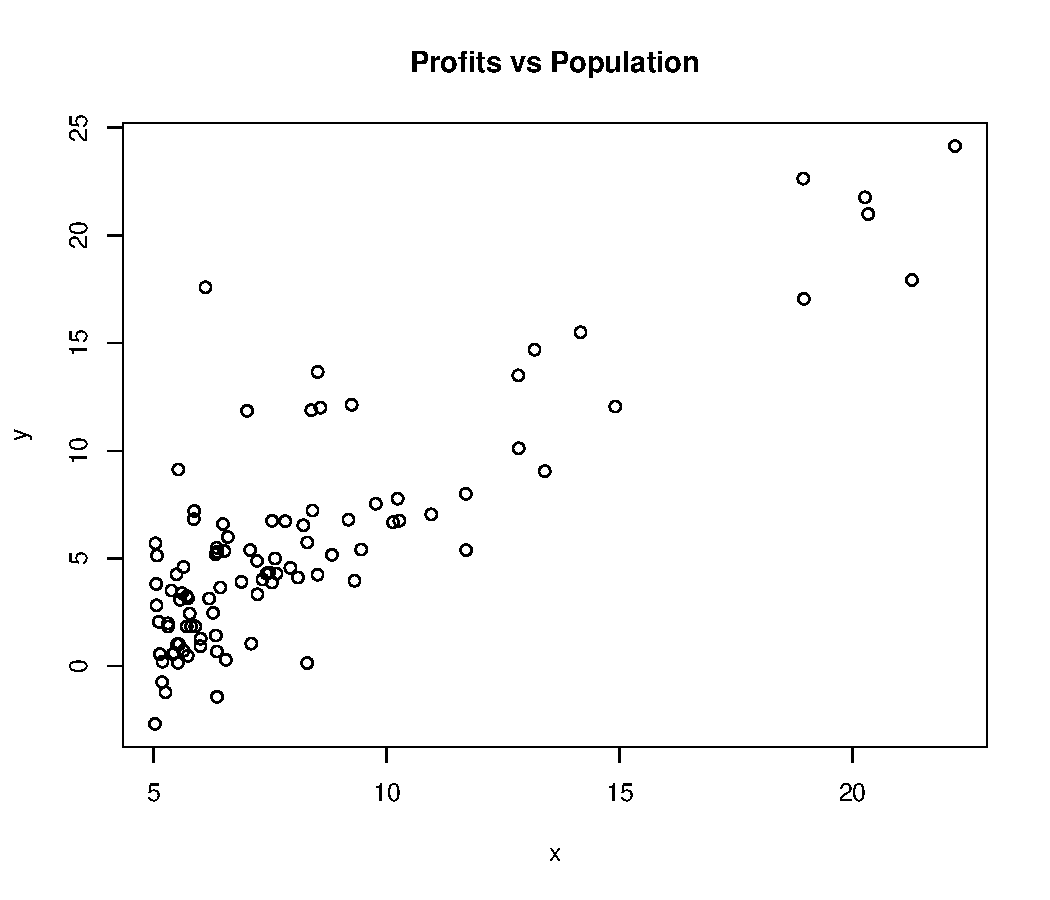
\includegraphics[width=\maxwidth]{figure/Regression} 

\end{knitrout}
The objective of the regression is to minimise the cost function.
\begin{equation}
J(\Theta_0, \Theta_1) = \frac{1}{2m} \sum_{i=1}^m (h_{\Theta}(X^{(i)} - y^{(i)}))^2
\end{equation}
Where the hypothesis is given by 
\begin{equation}
h_{\Theta}(x) = \Theta^Tx = \Theta_0 + \Theta_1x_1
\end{equation}
To take account of the intercept $\Theta_0$ an additional column of constants is added to $x$. 

\begin{knitrout}
\definecolor{shadecolor}{rgb}{0.969, 0.969, 0.969}\color{fgcolor}\begin{kframe}
\begin{alltt}
\hlcom{# Add ones to x}
\hlstd{x} \hlkwb{<-} \hlkwd{cbind}\hlstd{(}\hlnum{1}\hlstd{,x)}
\hlcom{# Initialise theta vector}
\hlstd{theta} \hlkwb{<-} \hlkwd{c}\hlstd{(}\hlnum{0}\hlstd{,}\hlnum{0}\hlstd{)}
\hlcom{# Number of observations}
\hlstd{m} \hlkwb{<-} \hlkwd{nrow}\hlstd{(x)}
\hlcom{# Calculate the cost}
\hlstd{cost} \hlkwb{<-} \hlkwd{sum}\hlstd{(((x}\hlopt\hlstd{theta)} \hlopt{-} \hlstd{y)}\hlopt{^}\hlnum{2}\hlstd{)}\hlopt{/}\hlstd{(}\hlnum{2}\hlopt{*}\hlstd{m)}
\hlstd{cost}
\end{alltt}
\begin{verbatim}
## [1] 32.07
\end{verbatim}
\end{kframe}
\end{knitrout}
The initial value is 32.07 (how do I take this from the chunk?).  Now 
\begin{knitrout}
\definecolor{shadecolor}{rgb}{0.969, 0.969, 0.969}\color{fgcolor}\begin{kframe}
\begin{alltt}
\hlcom{# Set learning parameter }
\hlstd{alpha} \hlkwb{<-} \hlnum{0.001}
\hlcom{#Number of iterations }
\hlstd{iterations} \hlkwb{<-} \hlnum{1500}
\hlcom{# updating thetas using gradient update }
\hlkwa{for}\hlstd{(i} \hlkwa{in} \hlnum{1}\hlopt{:}\hlstd{iterations)}
\hlstd{\{}
\hlstd{theta[}\hlnum{1}\hlstd{]} \hlkwb{<-} \hlstd{theta[}\hlnum{1}\hlstd{]} \hlopt{-} \hlstd{alpha} \hlopt{*} \hlstd{(}\hlnum{1}\hlopt{/}\hlstd{m)} \hlopt{*} \hlkwd{sum}\hlstd{(((x}\hlopt\hlstd{theta)}\hlopt{-} \hlstd{y))}
\hlstd{theta[}\hlnum{2}\hlstd{]} \hlkwb{<-} \hlstd{theta[}\hlnum{2}\hlstd{]} \hlopt{-} \hlstd{alpha} \hlopt{*} \hlstd{(}\hlnum{1}\hlopt{/}\hlstd{m)} \hlopt{*} \hlkwd{sum}\hlstd{(((x}\hlopt\hlstd{theta)}\hlopt{-} \hlstd{y)}\hlopt{*}\hlstd{x[,}\hlnum{2}\hlstd{])}
\hlstd{\}}
\hlcom{#Predict for areas of the 35,000 and 70,000 people }
\hlstd{predict1} \hlkwb{<-} \hlkwd{c}\hlstd{(}\hlnum{1}\hlstd{,}\hlnum{3.5}\hlstd{)} \hlopt \hlstd{theta}
\hlstd{predict2} \hlkwb{<-} \hlkwd{c}\hlstd{(}\hlnum{1}\hlstd{,}\hlnum{7}\hlstd{)} \hlopt \hlstd{theta}
\hlstd{predict1}
\end{alltt}
\begin{verbatim}
##       [,1]
## [1,] 2.247
\end{verbatim}
\begin{alltt}
\hlstd{predict2}
\end{alltt}
\begin{verbatim}
##       [,1]
## [1,] 5.356
\end{verbatim}
\begin{alltt}
\hlkwd{plot}\hlstd{(data}\hlopt{$}\hlstd{population} \hlopt{~} \hlstd{data}\hlopt{$}\hlstd{profit,} \hlkwc{main} \hlstd{=} \hlstr{"Profits vs Population"}\hlstd{)}
\hlkwd{abline}\hlstd{(theta,} \hlkwc{col} \hlstd{=} \hlstr{'red'}\hlstd{)}
\end{alltt}
\end{kframe}
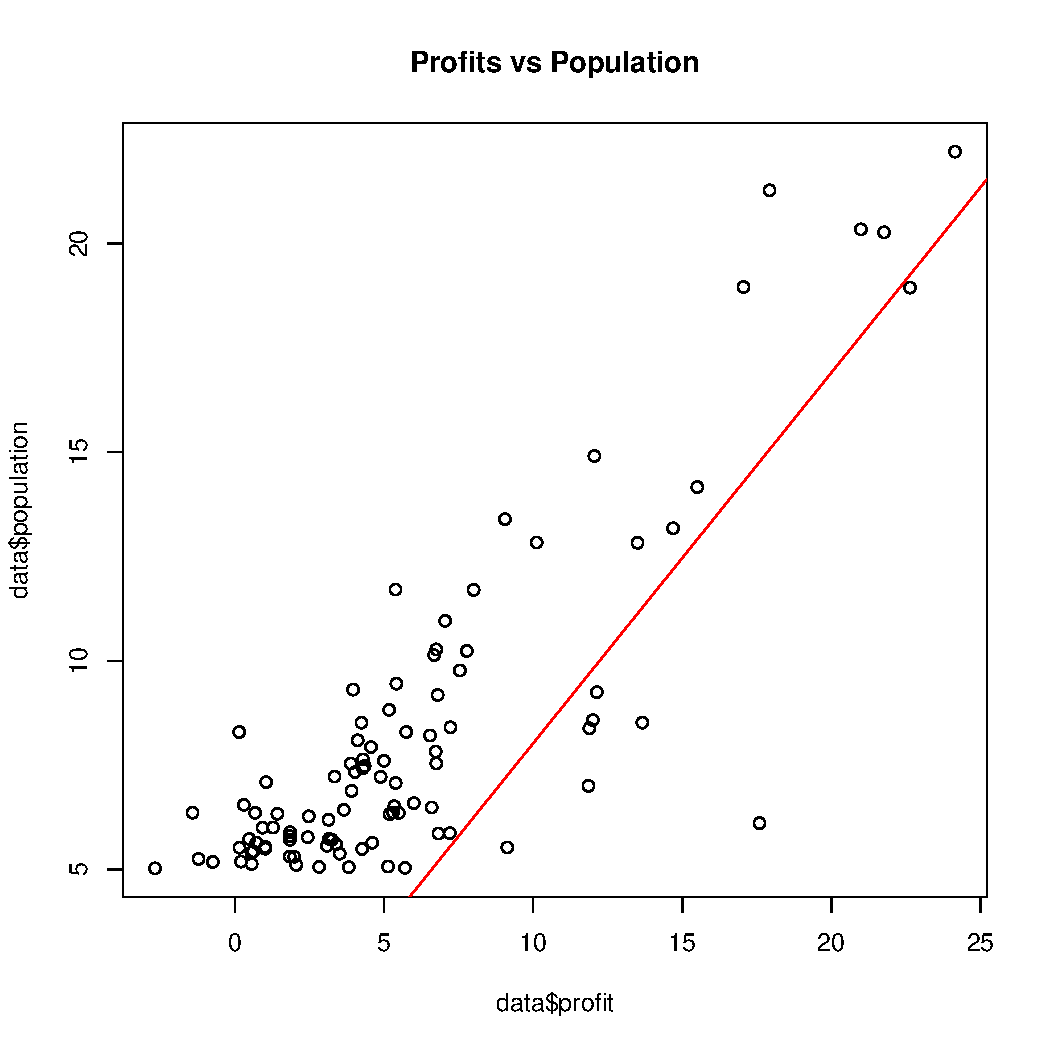
\includegraphics[width=\maxwidth]{figure/Regression3} 

\end{knitrout}
I think it is right, but....Needs to be looked at. 

\subsection{Adjusted R squared}
\href{http://davegiles.blogspot.ca/2013/05/when-will-adjusted-r-squared-increase.html}{Adjusted R squared} applied a penalty to the basic R squard to account for additional variables.  The equartion is 

\begin{equation}
R_A^2 = 1 - \left [ \frac{(n-1)}{(n-k)} \right ] [1 - R^2]
\end{equation}

Adding a regressor to the equation will increase (reduce)) the $R_A^"$ when the absolute value of the t-statistic is greater (less) than one. Adding a group of regressors to the model will reduce (increase) the $R_A^"$ when the absolute value of the F-statistic is greater than one.  

Proof \href{http://davegiles.blogspot.com/2014/04/proof-of-result-about-adjusted.html}{http://davegiles.blogspot.com/2014/04/proof-of-result-about-adjusted.html}

\subsection{Monte Carlo Simulation}
This comes from \href{http://blog.revolutionanalytics.com/2014/04/quantitative-finance-applications-in-r-5.html}{Revoluitionary Analytics}.  The analysis is in annual terms.  

\begin{equation}
\mu \Delta t + \sigma Z \sqrt{\Delta t}
\end{equation}

where $\mu$ is the drift or average annual return, Z is a standard Normal random variable, t is measured in years so for monthly returns $\Delta t$ equals $\frac{1}{12}$.























